This section presents a detailed overview of the program flow of the final interrupt-oriented paddle program.

\begin{figure}
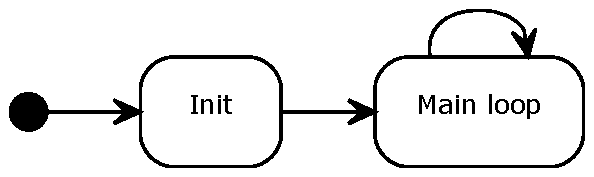
\includegraphics[width = \textwidth]{description-and-methodology/program-flow/main-program-flow.pdf}
\caption{Main superficial program flow}
\label{fig:hist}
\end{figure}

\begin{figure}
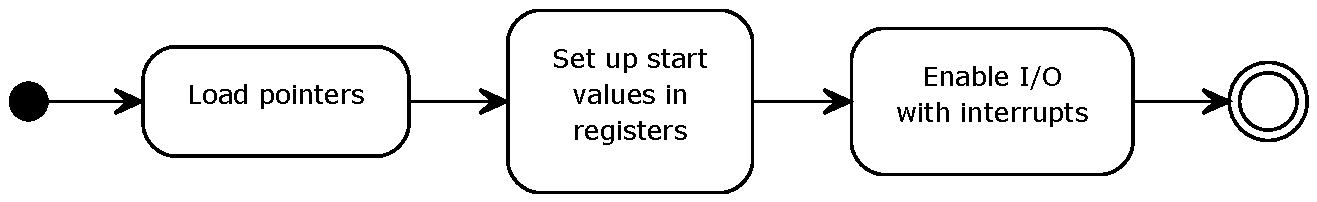
\includegraphics[width = \textwidth]{description-and-methodology/program-flow/init.pdf}
\caption{Initialization}
\label{fig:hist}
\end{figure}

\begin{figure}
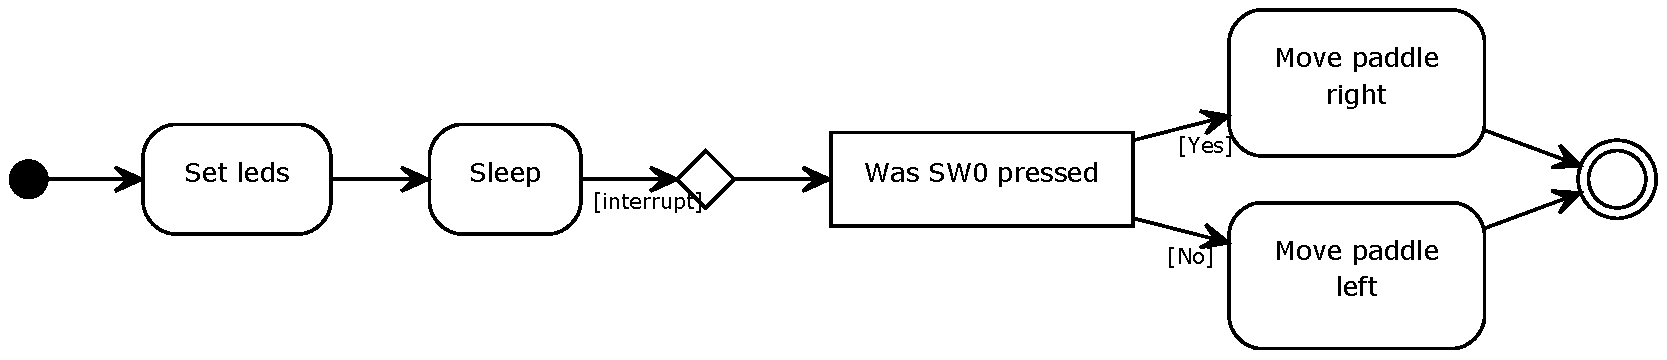
\includegraphics[width = \textwidth]{description-and-methodology/program-flow/main-loop.pdf}
\caption{Main loop}
\label{fig:hist}
\end{figure}

\begin{figure}
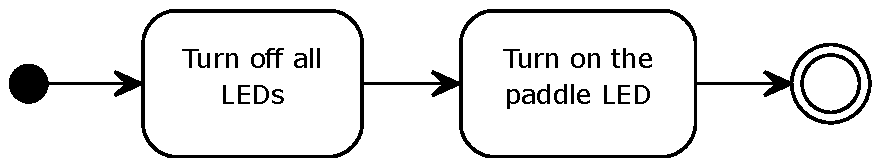
\includegraphics[width = \textwidth]{description-and-methodology/program-flow/set-leds.pdf}
\caption{Set leds subroutine}
\label{fig:hist}
\end{figure}

\begin{figure}
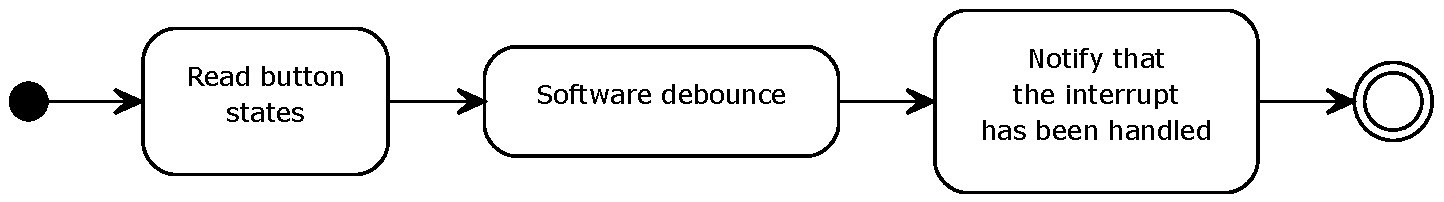
\includegraphics[width = \textwidth]{description-and-methodology/program-flow/button-interrupt-routine.pdf}
\caption{Button interrupt routine}
\label{fig:hist}
\end{figure}

\begin{figure}
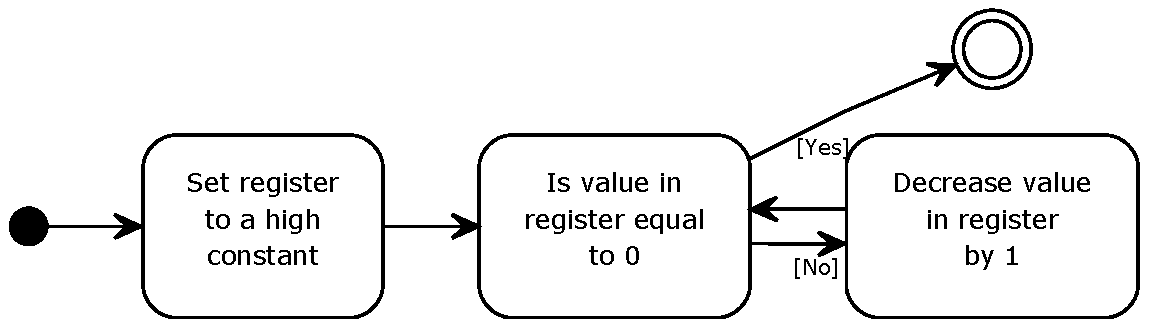
\includegraphics[width = \textwidth]{description-and-methodology/program-flow/debounce.pdf}
\caption{Debounce subroutine}
\label{fig:hist}
\end{figure}

\begin{figure}
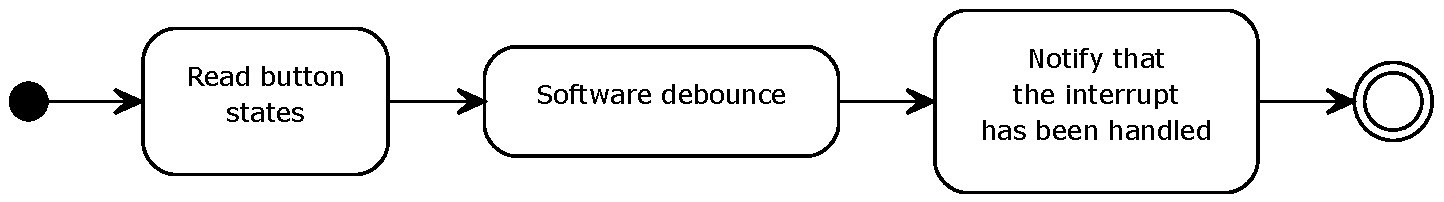
\includegraphics[width = \textwidth]{description-and-methodology/program-flow/read-buttons.pdf}
\caption{Read buttons subroutine}
\label{fig:hist}
\end{figure}

\begin{figure}
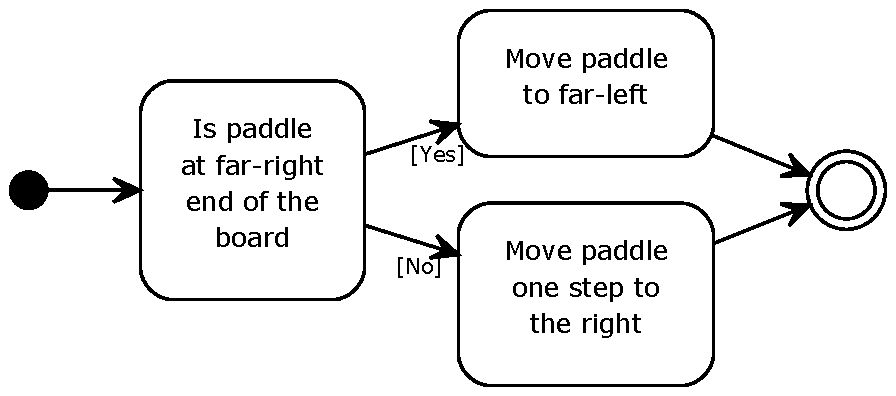
\includegraphics[width = \textwidth]{description-and-methodology/program-flow/move-paddle-right.pdf}
\caption{Move paddle right subroutine}
\label{fig:hist}
\end{figure}

\begin{figure}
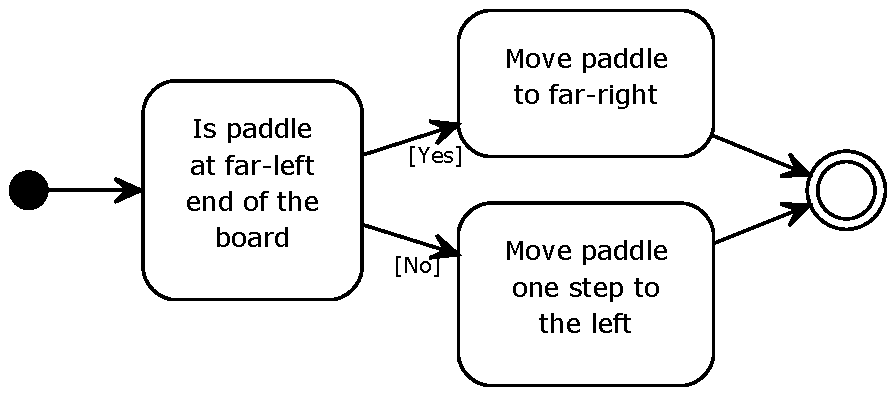
\includegraphics[width = \textwidth]{description-and-methodology/program-flow/move-paddle-left.pdf}
\caption{Move paddle left subroutine (analogous to move paddle right subroutine, but included for completeness}
\label{fig:hist}
\end{figure}

